\documentclass[12pt,a4paper]{article}
\usepackage[utf8]{inputenc}
\usepackage[indonesian]{babel}
\usepackage{geometry}
\usepackage{booktabs}
\usepackage{amsmath}
\usepackage{amssymb}
\usepackage{float}
\usepackage{array}
\usepackage{xcolor}
\usepackage{colortbl}
\usepackage{graphicx}
\usepackage{hyperref}
\usepackage{fancyhdr}
\usepackage{titlesec}
\usepackage{caption}
\usepackage{subcaption}
\usepackage{longtable}
\usepackage{multirow}
\usepackage{makecell}
\usepackage{parskip}

\geometry{left=3cm, right=2.5cm, top=3cm, bottom=2.5cm}

\definecolor{headerblue}{RGB}{23, 62, 125}
\definecolor{rowlight}{RGB}{235, 242, 255}

\pagestyle{fancy}
\fancyhf{}
\fancyhead[L]{\footnotesize\textcolor{headerblue}{\textbf{Statistika Deskriptif Detail}}}
\fancyhead[R]{\footnotesize\textcolor{gray}{Valuasi Harga Rumah DKI Jakarta 2024}}
\fancyfoot[C]{\thepage}
\renewcommand{\headrulewidth}{0.5pt}

\titleformat{\section}{\Large\bfseries\color{headerblue}}{\thesection.}{0.5em}{}
\titleformat{\subsection}{\large\bfseries\color{headerblue!80!black}}{\thesubsection.}{0.5em}{}
\titleformat{\subsubsection}{\normalsize\bfseries\color{headerblue!60!black}}{\thesubsubsection.}{0.5em}{}

\captionsetup{font=small,labelfont=bf}

\hypersetup{
  colorlinks=true,
  linkcolor=headerblue,
  urlcolor=blue,
  pdfauthor={Ammar Hanafi, Norman Mowlana Aziz, Kirono Dwi Saputro},
  pdftitle={Statistika Deskriptif Detail: Valuasi Harga Rumah DKI Jakarta 2024},
}

\begin{document}

\begin{titlepage}
\centering
\vspace*{1.5cm}
{\color{headerblue}\rule{\linewidth}{3pt}}\\[0.4cm]
{\LARGE\bfseries\color{headerblue} STATISTIKA DESKRIPTIF DETAIL}\\[0.3cm]
{\Large\bfseries Eksplorasi Karakteristik Data Uji}\\[0.15cm]
{\color{headerblue}\rule{\linewidth}{1pt}}\\[0.5cm]
{\large\textit{Analisis Geographically Weighted Regression (GWR)}\\
\textit{pada Kasus Valuasi Harga Rumah di DKI Jakarta 2024}}\\[2cm]

\begin{tabular}{c}
{\normalsize\textbf{AMMAR HANAFI (2206051582)}} \\[3pt]
{\normalsize\textbf{NORMAN MOWLANA AZIZ (2206025470)}} \\[3pt]
{\normalsize\textbf{KIRONO DWI SAPUTRO (2106656365)}} \\
\end{tabular}

\vfill
{\normalsize\textbf{PROGRAM STUDI SARJANA STATISTIKA}\\
\textbf{FAKULTAS MATEMATIKA DAN ILMU PENGETAHUAN ALAM}\\
\textbf{UNIVERSITAS INDONESIA}\\[0.3cm]
\textbf{DEPOK --- JUNI 2026}}\\[0.5cm]
{\color{headerblue}\rule{\linewidth}{2pt}}
\end{titlepage}

\tableofcontents
\newpage

%============================================================
\section{Pendahuluan dan Deskripsi Dataset}
%============================================================

Dokumen ini merupakan lampiran analitik khusus yang menyajikan eksplorasi statistik
deskriptif secara menyeluruh atas dataset harga rumah di DKI Jakarta tahun 2024.
Data bersumber dari \textit{GeoJSON dataset} pasar sekunder perumahan DKI Jakarta
yang telah melalui tahap \textit{data cleaning}. Total observasi yang valid adalah
\textbf{1.079 unit rumah}.

\subsection{Deskripsi Variabel Penelitian}

\begin{table}[H]
\centering
\caption{Definisi Operasional Variabel Penelitian}
\label{tab:var_def}
\small
\begin{tabular}{clll}
\toprule
\rowcolor{headerblue}
\textcolor{white}{\textbf{Notasi}} & \textcolor{white}{\textbf{Nama Variabel}} & \textcolor{white}{\textbf{Satuan}} & \textcolor{white}{\textbf{Peran}} \\
\midrule
\rowcolor{rowlight}
$Y$   & Harga Rumah         & Miliar Rp & Dependen                   \\
$X_1$ & Luas Bangunan       & m$^2$     & Independen (Fisik)         \\
\rowcolor{rowlight}
$X_2$ & Luas Tanah/Kaveling & m$^2$     & Independen (Fisik)         \\
$X_3$ & Jumlah Kamar        & Unit      & Independen (Fisik)         \\
\rowcolor{rowlight}
$X_4$ & Jarak ke Monas      & km        & Independen (Spasial)       \\
$X_5$ & Jarak ke Sekolah    & km        & Independen (Aksesibilitas) \\
\rowcolor{rowlight}
$X_6$ & Jarak ke Rumah Sakit & km       & Independen (Aksesibilitas) \\
$X_7$ & Jarak ke Jalan Utama & km       & Independen (Aksesibilitas) \\
\bottomrule
\end{tabular}
\end{table}

\newpage
%============================================================
\section{Statistik Ringkasan Komprehensif}
%============================================================

\subsection{Ukuran Pemusatan dan Posisi}

\begin{table}[H]
\centering
\caption{Lima Angka Ringkasan, Rata-rata, dan Standar Deviasi}
\label{tab:summary1}
\small
\setlength{\tabcolsep}{5.5pt}
\begin{tabular}{lrrrrrrrr}
\toprule
\rowcolor{headerblue}
\textcolor{white}{\textbf{Var}} &
\textcolor{white}{\textbf{$n$}} &
\textcolor{white}{\textbf{Min}} &
\textcolor{white}{\textbf{$Q_1$}} &
\textcolor{white}{\textbf{Median}} &
\textcolor{white}{\textbf{Mean}} &
\textcolor{white}{\textbf{$Q_3$}} &
\textcolor{white}{\textbf{Max}} &
\textcolor{white}{\textbf{Std.Dev}} \\
\midrule
\rowcolor{rowlight}
Harga (Y) & 1079 & 0.3650 & 1.9700 & 3.5000 & 9.7813 & 9.2500 & 221.000 & 18.8377 \\
LB (X1) & 1079 & 36.0000 & 105.500 & 192.000 & 269.577 & 335.500 & 4,850.00 & 279.736 \\
\rowcolor{rowlight}
LT (X2) & 1079 & 19.0000 & 87.5000 & 132.000 & 266.057 & 301.000 & 10,847 & 448.825 \\
KT (X3) & 1079 & 1.0000 & 3.0000 & 3.0000 & 3.7025 & 4.0000 & 17.0000 & 1.4688 \\
\rowcolor{rowlight}
Monas (X4) & 1079 & 0.2133 & 6.4334 & 9.5226 & 9.5852 & 12.2242 & 21.2055 & 3.9379 \\
Sekolah (X5) & 1079 & 0.0000 & 0.5387 & 1.0328 & 1.4448 & 1.7056 & 8.1757 & 1.5061 \\
\rowcolor{rowlight}
RS (X6) & 1079 & 0.0000 & 0.9570 & 1.6024 & 2.1459 & 2.6514 & 8.9700 & 1.8226 \\
Jalan (X7) & 1079 & 0.0000 & 0.0055 & 0.0119 & 0.0159 & 0.0218 & 0.2845 & 0.0167 \\
\bottomrule
\end{tabular}
\end{table}

\noindent\textbf{Keterangan:} $Q_1$ = Kuartil ke-1 (persentil ke-25),
$Q_3$ = Kuartil ke-3 (persentil ke-75).
Nilai mean $Y$ yang jauh di atas median mengkonfirmasi distribusi harga yang menceng
kanan (\textit{positively skewed}) --- ciri khas pasar properti heterogen.

\subsection{Ukuran Keragaman dan Dispersi}

\begin{table}[H]
\centering
\caption{Ukuran Dispersi dan Keragaman Data}
\label{tab:dispersi}
\small
\setlength{\tabcolsep}{6pt}
\begin{tabular}{lrrrrrr}
\toprule
\rowcolor{headerblue}
\textcolor{white}{\textbf{Var}} &
\textcolor{white}{\textbf{Varian ($s^2$)}} &
\textcolor{white}{\textbf{CV (\%)}} &
\textcolor{white}{\textbf{IQR}} &
\textcolor{white}{\textbf{Range}} &
\textcolor{white}{\textbf{Skewness}} &
\textcolor{white}{\textbf{Kurtosis*}} \\
\midrule
\rowcolor{rowlight}
Harga (Y) & 354.861 & 192.589\% & 7.2800 & 220.635 & 5.8146 & 48.0383 \\
LB (X1) & 78,252 & 103.768\% & 230.000 & 4,814.00 & 5.6303 & 70.5120 \\
\rowcolor{rowlight}
LT (X2) & 201,444 & 168.695\% & 213.500 & 10,828 & 13.1932 & 289.013 \\
KT (X3) & 2.16 & 39.67\% & 1.0000 & 16.0000 & 2.6102 & 15.3124 \\
\rowcolor{rowlight}
Monas (X4) & 15.51 & 41.08\% & 5.7908 & 20.9922 & 0.2972 & -0.1039 \\
Sekolah (X5) & 2.27 & 104.240\% & 1.1669 & 8.1757 & 2.4798 & 6.4839 \\
\rowcolor{rowlight}
RS (X6) & 3.32 & 84.93\% & 1.6944 & 8.9700 & 1.6344 & 2.3382 \\
Jalan (X7) & 0.00 & 104.705\% & 0.0162 & 0.2845 & 5.2608 & 65.5754 \\
\bottomrule
\multicolumn{7}{l}{\footnotesize *Excess Kurtosis (Normal$=0$).
  Positif $\Rightarrow$ leptokurtik (ekor tebal), Negatif $\Rightarrow$ platikurtik.}
\end{tabular}
\end{table}

\noindent\textbf{Interpretasi CV:} Koefisien Variasi (CV) mengukur keragaman relatif terhadap
rata-rata. CV $>30\%$ = keragaman \textit{tinggi}. Seluruh variabel memiliki CV relatif
tinggi, mencerminkan heterogenitas data perumahan Jakarta yang nyata.

\subsection{Klasifikasi Bentuk Distribusi}

\begin{table}[H]
\centering
\caption{Klasifikasi Distribusi Berdasarkan Momen Ketiga dan Keempat}
\label{tab:distribusi}
\small
\begin{tabular}{lrrlr}
\toprule
\rowcolor{headerblue}
\textcolor{white}{\textbf{Var}} &
\textcolor{white}{\textbf{Skewness}} &
\textcolor{white}{\textbf{Kurtosis}} &
\textcolor{white}{\textbf{Kemencengan}} &
\textcolor{white}{\textbf{Ketinggian Puncak}} \\
\midrule
\rowcolor{rowlight}
Harga (Y) & 5.8146 & 48.0383 & \textit{Right-Skewed Kuat} & Leptokurtik \\
LB (X1) & 5.6303 & 70.5120 & \textit{Right-Skewed Kuat} & Leptokurtik \\
\rowcolor{rowlight}
LT (X2) & 13.1932 & 289.013 & \textit{Right-Skewed Kuat} & Leptokurtik \\
KT (X3) & 2.6102 & 15.3124 & \textit{Right-Skewed Kuat} & Leptokurtik \\
\rowcolor{rowlight}
Monas (X4) & 0.2972 & -0.1039 & Mendekati Simetris & Mesokurtik \\
Sekolah (X5) & 2.4798 & 6.4839 & \textit{Right-Skewed Kuat} & Leptokurtik \\
\rowcolor{rowlight}
RS (X6) & 1.6344 & 2.3382 & \textit{Right-Skewed Kuat} & Mesokurtik \\
Jalan (X7) & 5.2608 & 65.5754 & \textit{Right-Skewed Kuat} & Leptokurtik \\
\bottomrule
\end{tabular}
\end{table}

\newpage
%============================================================
\section{Analisis Per Variabel}
%============================================================

Berikut disajikan analisis statistik deskriptif mendalam per variabel, meliputi
tabel statistik lengkap dan interpretasi analitik.


\subsection{\texorpdfstring{$Y$}{Y} --- Harga Rumah (Miliar Rp)}
\begin{center}
\begin{tabular}{|l|r||l|r|}
\hline
\textbf{Statistik} & \textbf{Nilai} & \textbf{Statistik} & \textbf{Nilai} \\
\hline
$n$ (Observasi) & 1079 & Rentang (Range) & 220.635 Miliar Rp \\
Minimum & 0.3650 Miliar Rp & IQR ($Q_3 - Q_1$) & 7.2800 Miliar Rp \\
$Q_1$ (Kuartil 1) & 1.9700 Miliar Rp & Standar Deviasi & 18.8377 Miliar Rp \\
Median ($Q_2$) & 3.5000 Miliar Rp & Varian & 354.861 \\
Rata-rata ($\bar{x}$) & 9.7813 Miliar Rp & Koef.~Variasi & 192.589\% \\
$Q_3$ (Kuartil 3) & 9.2500 Miliar Rp & Skewness & 5.8146 \\
Maksimum & 221.000 Miliar Rp & Kurtosis (Excess) & 48.0383 \\
\hline
\end{tabular}
\end{center}

\noindent Variabel dependen $Y$ (harga rumah) memiliki distribusi yang sangat menceng kanan (\textit{right-skewed}) dengan nilai maksimum mencapai \textbf{Rp221 miliar}, sementara median jauh di bawah rata-rata. Hal ini menunjukkan adanya outlier ekstrem berupa properti mewah di Jakarta Selatan dan Pusat. Koefisien variasi (CV) yang sangat tinggi menegaskan heterogenitas kelas harga properti Jakarta.


\subsection{\texorpdfstring{$X_1$ --- Luas Bangunan (m\textsuperscript{2})}{X1 --- Luas Bangunan (m2)}}
\begin{center}
\begin{tabular}{|l|r||l|r|}
\hline
\textbf{Statistik} & \textbf{Nilai} & \textbf{Statistik} & \textbf{Nilai} \\
\hline
$n$ (Observasi) & 1079 & Rentang (Range) & 4,814.00 m$^2$ \\
Minimum & 36.0000 m$^2$ & IQR ($Q_3 - Q_1$) & 230.000 m$^2$ \\
$Q_1$ (Kuartil 1) & 105.500 m$^2$ & Standar Deviasi & 279.736 m$^2$ \\
Median ($Q_2$) & 192.000 m$^2$ & Varian & 78,252 \\
Rata-rata ($\bar{x}$) & 269.577 m$^2$ & Koef.~Variasi & 103.768\% \\
$Q_3$ (Kuartil 3) & 335.500 m$^2$ & Skewness & 5.6303 \\
Maksimum & 4,850.00 m$^2$ & Kurtosis (Excess) & 70.5120 \\
\hline
\end{tabular}
\end{center}

\noindent Luas bangunan ($X_1$) berkisar antara \textbf{36 m$^2$} (rumah tipe kecil) hingga \textbf{4.850 m$^2$} (vila/mansion). Skewness positif tinggi mengindikasikan adanya properti berukuran sangat besar yang membentuk ekor distribusi panjang.


\subsection{\texorpdfstring{$X_2$ --- Luas Tanah (m\textsuperscript{2})}{X2 --- Luas Tanah (m2)}}
\begin{center}
\begin{tabular}{|l|r||l|r|}
\hline
\textbf{Statistik} & \textbf{Nilai} & \textbf{Statistik} & \textbf{Nilai} \\
\hline
$n$ (Observasi) & 1079 & Rentang (Range) & 10,828 m$^2$ \\
Minimum & 19.0000 m$^2$ & IQR ($Q_3 - Q_1$) & 213.500 m$^2$ \\
$Q_1$ (Kuartil 1) & 87.5000 m$^2$ & Standar Deviasi & 448.825 m$^2$ \\
Median ($Q_2$) & 132.000 m$^2$ & Varian & 201,444 \\
Rata-rata ($\bar{x}$) & 266.057 m$^2$ & Koef.~Variasi & 168.695\% \\
$Q_3$ (Kuartil 3) & 301.000 m$^2$ & Skewness & 13.1932 \\
Maksimum & 10,847 m$^2$ & Kurtosis (Excess) & 289.013 \\
\hline
\end{tabular}
\end{center}

\noindent Luas kaveling tanah ($X_2$) menunjukkan dispersi tertinggi di antara variabel fisik, dengan standar deviasi \textbf{448,8 m$^2$}. Fenomena ini lazim di Jakarta karena variasi ekstrem antara rumah tapak kecil dan hunian besar di kawasan premium (Pondok Indah, Menteng).


\subsection{\texorpdfstring{$X_3$}{X3} --- Jumlah Kamar}
\begin{center}
\begin{tabular}{|l|r||l|r|}
\hline
\textbf{Statistik} & \textbf{Nilai} & \textbf{Statistik} & \textbf{Nilai} \\
\hline
$n$ (Observasi) & 1079 & Rentang (Range) & 16.0000 Kamar \\
Minimum & 1.0000 Kamar & IQR ($Q_3 - Q_1$) & 1.0000 Kamar \\
$Q_1$ (Kuartil 1) & 3.0000 Kamar & Standar Deviasi & 1.4688 Kamar \\
Median ($Q_2$) & 3.0000 Kamar & Varian & 2.16 \\
Rata-rata ($\bar{x}$) & 3.7025 Kamar & Koef.~Variasi & 39.67\% \\
$Q_3$ (Kuartil 3) & 4.0000 Kamar & Skewness & 2.6102 \\
Maksimum & 17.0000 Kamar & Kurtosis (Excess) & 15.3124 \\
\hline
\end{tabular}
\end{center}

\noindent Jumlah kamar ($X_3$) memiliki distribusi paling mendekati simetris di antara variabel fisik, dengan median \textbf{3 kamar}. Rentang 1--17 kamar mencerminkan segmentasi pasar dari unit studio hingga gedung residensial besar.


\subsection{\texorpdfstring{$X_4$}{X4} --- Jarak ke Monas (km)}
\begin{center}
\begin{tabular}{|l|r||l|r|}
\hline
\textbf{Statistik} & \textbf{Nilai} & \textbf{Statistik} & \textbf{Nilai} \\
\hline
$n$ (Observasi) & 1079 & Rentang (Range) & 20.9922 km \\
Minimum & 0.2133 km & IQR ($Q_3 - Q_1$) & 5.7908 km \\
$Q_1$ (Kuartil 1) & 6.4334 km & Standar Deviasi & 3.9379 km \\
Median ($Q_2$) & 9.5226 km & Varian & 15.51 \\
Rata-rata ($\bar{x}$) & 9.5852 km & Koef.~Variasi & 41.08\% \\
$Q_3$ (Kuartil 3) & 12.2242 km & Skewness & 0.2972 \\
Maksimum & 21.2055 km & Kurtosis (Excess) & -0.1039 \\
\hline
\end{tabular}
\end{center}

\noindent Jarak ke Monas ($X_4$) sebagai proksi \textit{centrality} memiliki rata-rata \textbf{9,57 km}. Distribusinya paling mendekati normal (skewness mendekati 0) di antara semua variabel, mencerminkan persebaran properti yang cukup merata secara radial dari pusat kota.


\subsection{\texorpdfstring{$X_5$}{X5} --- Jarak ke Sekolah (km)}
\begin{center}
\begin{tabular}{|l|r||l|r|}
\hline
\textbf{Statistik} & \textbf{Nilai} & \textbf{Statistik} & \textbf{Nilai} \\
\hline
$n$ (Observasi) & 1079 & Rentang (Range) & 8.1757 km \\
Minimum & 0.0000 km & IQR ($Q_3 - Q_1$) & 1.1669 km \\
$Q_1$ (Kuartil 1) & 0.5387 km & Standar Deviasi & 1.5061 km \\
Median ($Q_2$) & 1.0328 km & Varian & 2.27 \\
Rata-rata ($\bar{x}$) & 1.4448 km & Koef.~Variasi & 104.240\% \\
$Q_3$ (Kuartil 3) & 1.7056 km & Skewness & 2.4798 \\
Maksimum & 8.1757 km & Kurtosis (Excess) & 6.4839 \\
\hline
\end{tabular}
\end{center}

\noindent Jarak ke sekolah ($X_5$) memiliki nilai minimum 0 km dan maksimum \textbf{8,18 km}. Rata-rata \textbf{1,44 km} menunjukkan bahwa sebagian besar properti relatif dekat dengan fasilitas pendidikan. Skewness positif mengindikasikan sebaran terkonsentrasi di jarak dekat.


\subsection{\texorpdfstring{$X_6$}{X6} --- Jarak ke RS (km)}
\begin{center}
\begin{tabular}{|l|r||l|r|}
\hline
\textbf{Statistik} & \textbf{Nilai} & \textbf{Statistik} & \textbf{Nilai} \\
\hline
$n$ (Observasi) & 1079 & Rentang (Range) & 8.9700 km \\
Minimum & 0.0000 km & IQR ($Q_3 - Q_1$) & 1.6944 km \\
$Q_1$ (Kuartil 1) & 0.9570 km & Standar Deviasi & 1.8226 km \\
Median ($Q_2$) & 1.6024 km & Varian & 3.32 \\
Rata-rata ($\bar{x}$) & 2.1459 km & Koef.~Variasi & 84.93\% \\
$Q_3$ (Kuartil 3) & 2.6514 km & Skewness & 1.6344 \\
Maksimum & 8.9700 km & Kurtosis (Excess) & 2.3382 \\
\hline
\end{tabular}
\end{center}

\noindent Jarak ke rumah sakit ($X_6$) berkorelasi sangat tinggi dengan $X_5$ ($r=0{,}747$), menandakan pola klasterisasi fasilitas publik. Variabel ini memiliki pengaruh negatif signifikan terhadap harga pada model OLS, mengindikasikan bahwa properti yang jauh dari RS cenderung lebih murah.


\subsection{\texorpdfstring{$X_7$}{X7} --- Jarak ke Jalan Utama (km)}
\begin{center}
\begin{tabular}{|l|r||l|r|}
\hline
\textbf{Statistik} & \textbf{Nilai} & \textbf{Statistik} & \textbf{Nilai} \\
\hline
$n$ (Observasi) & 1079 & Rentang (Range) & 0.2845 km \\
Minimum & 0.0000 km & IQR ($Q_3 - Q_1$) & 0.0162 km \\
$Q_1$ (Kuartil 1) & 0.0055 km & Standar Deviasi & 0.0167 km \\
Median ($Q_2$) & 0.0119 km & Varian & 0.00 \\
Rata-rata ($\bar{x}$) & 0.0159 km & Koef.~Variasi & 104.705\% \\
$Q_3$ (Kuartil 3) & 0.0218 km & Skewness & 5.2608 \\
Maksimum & 0.2845 km & Kurtosis (Excess) & 65.5754 \\
\hline
\end{tabular}
\end{center}

\noindent Jarak ke jalan utama ($X_7$) memiliki skala sangat kecil (rata-rata $\approx$0,016 km = 16 meter), menunjukkan hampir seluruh properti berada sangat dekat dengan akses jalan utama. CV ekstrem mengindikasikan distribusi sangat skewed dengan sebagian kecil properti terisolasi jauh dari akses jalan.

\newpage
%============================================================
\section{Visualisasi Distribusi dan Hubungan Spasial}
%============================================================

Visualisasi di bawah ini memberikan gambaran grafis mengenai persebaran data (Boxplot) dan hubungan antar variabel secara simultan (Pairplot).

\subsection{Boxplot Distribusi Variabel}
Boxplot digunakan untuk mengidentifikasi rentang data, kuartil, dan keberadaan pencilan (\textit{outliers}) secara visual. 

\begin{figure}[H]
    \centering
    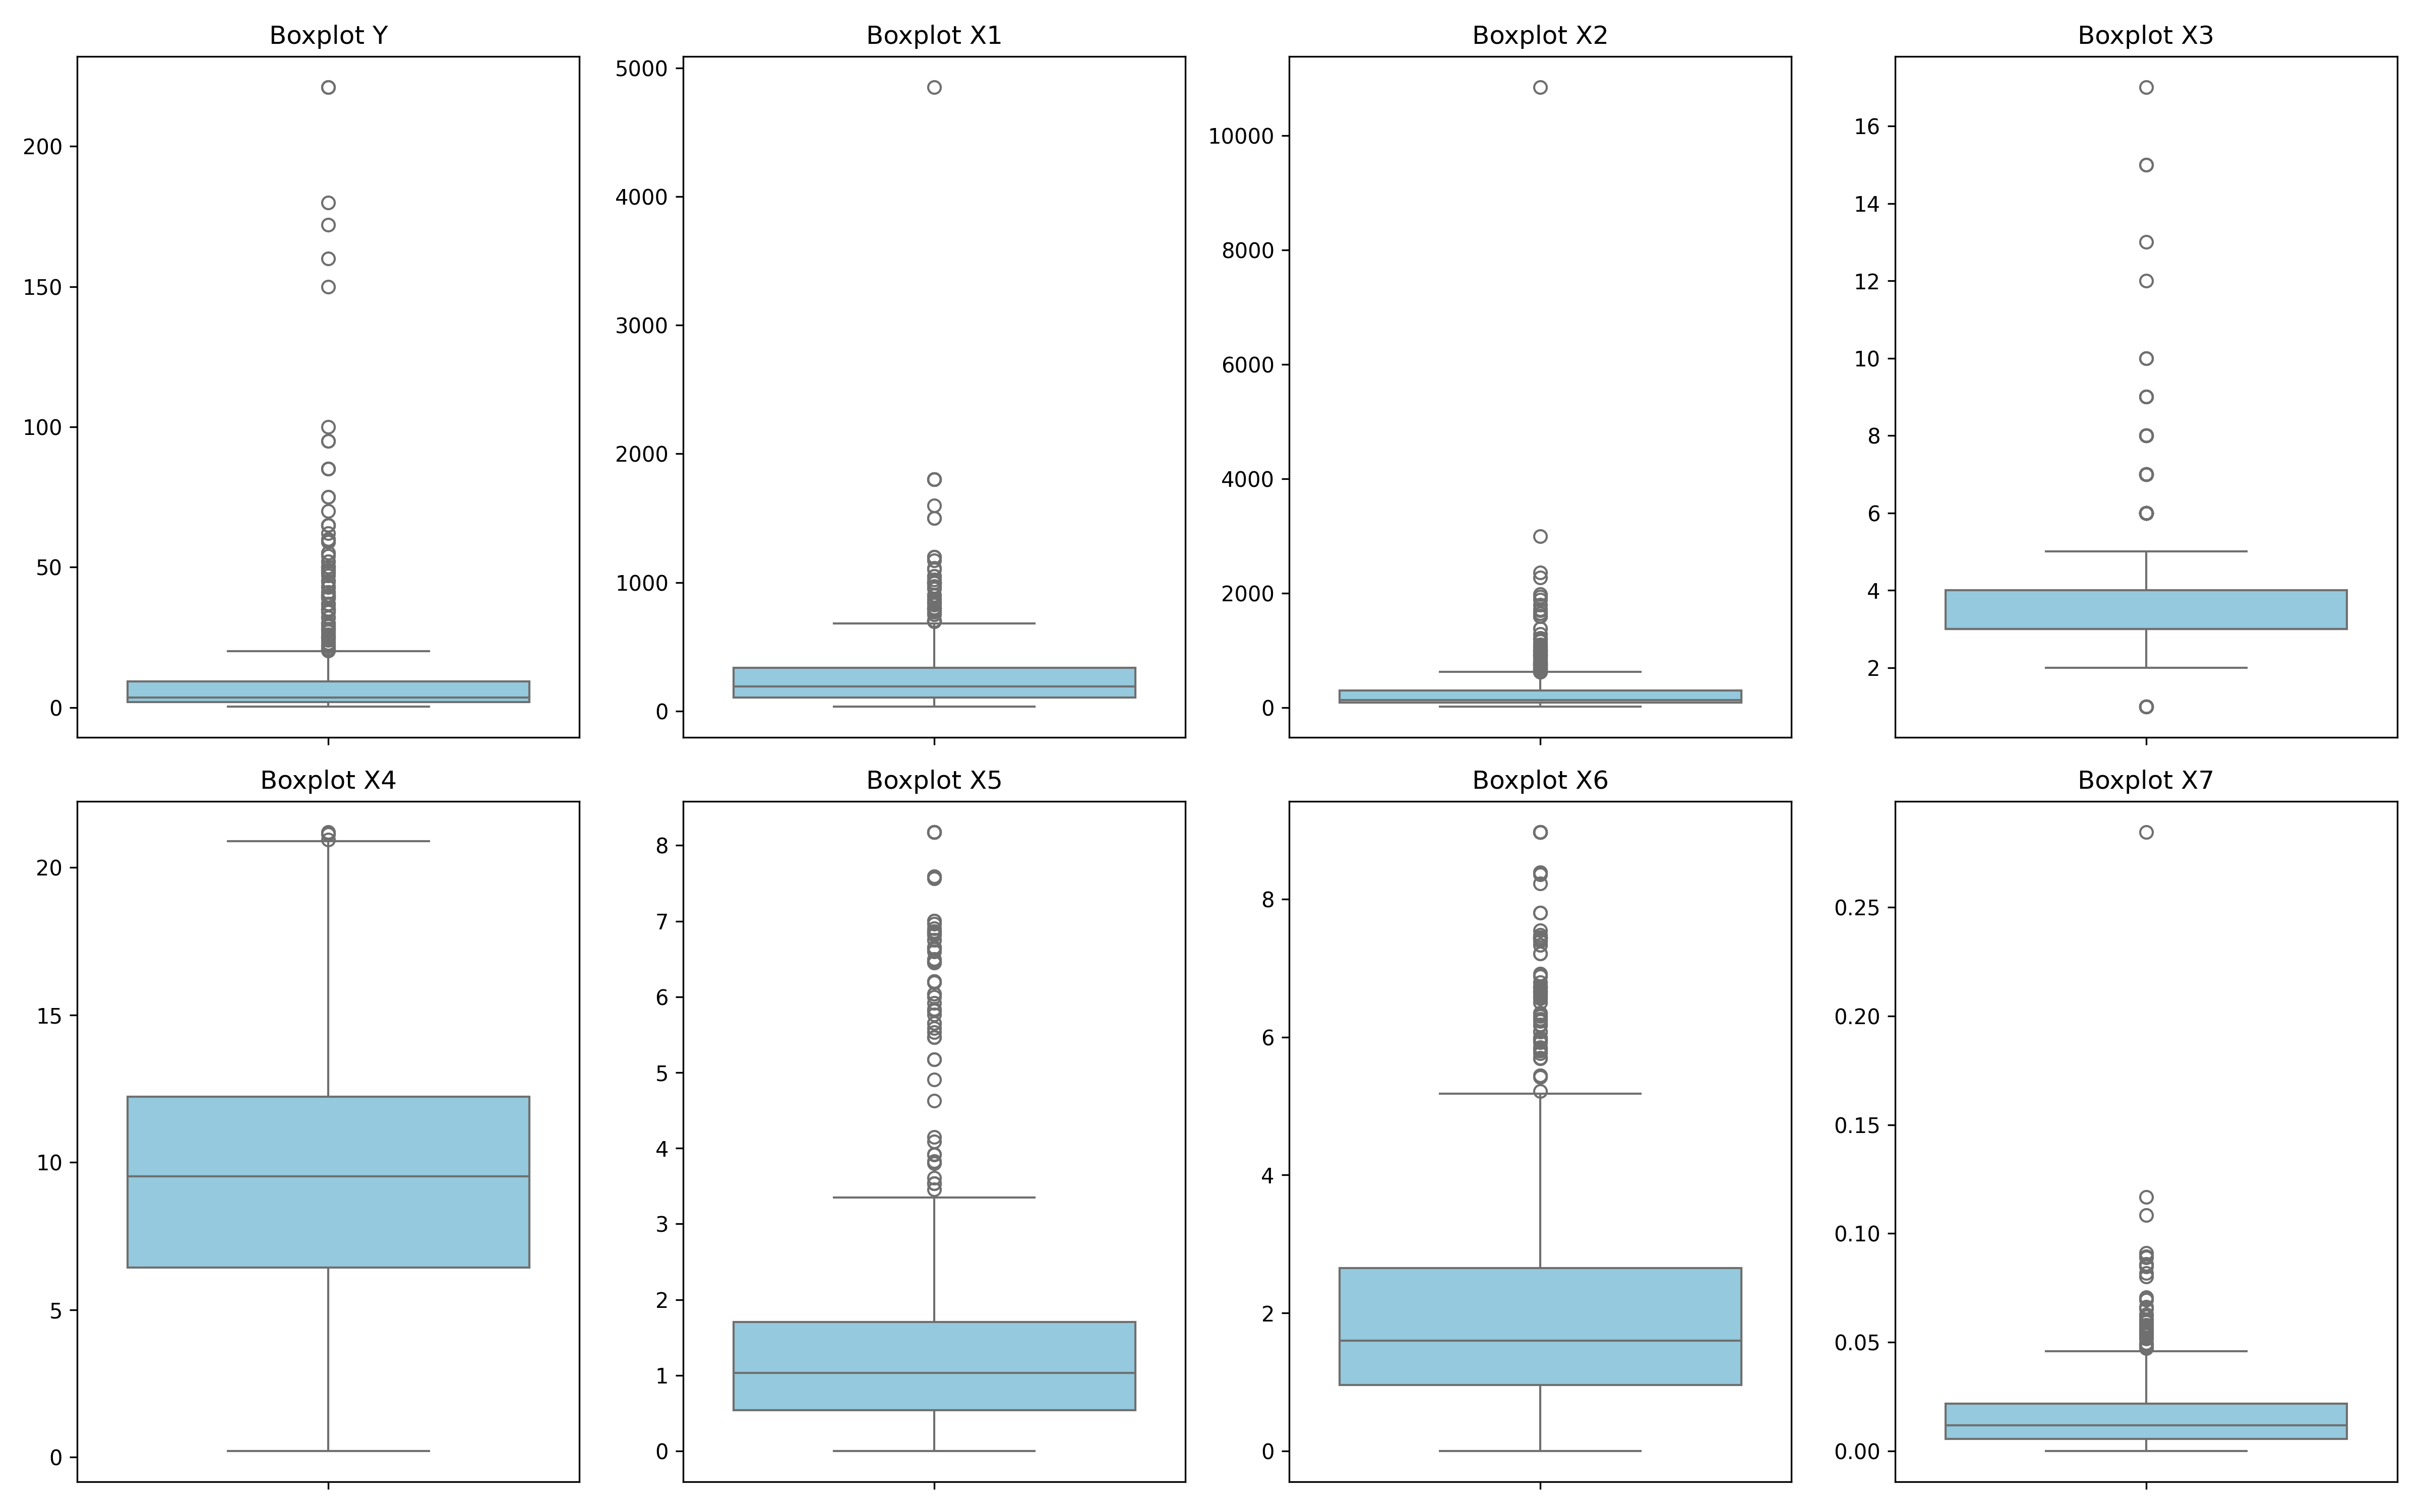
\includegraphics[width=\textwidth]{boxplot_deskriptif.png}
    \caption{Boxplot Seluruh Variabel Penelitian (Skala Mandiri)}
    \label{fig:boxplot_all}
\end{figure}

\subsection{Pairplot (Matrix Scatter Plot)}
Pairplot menyajikan matriks plot sebar untuk melihat hubungan linear antar pasangan variabel serta estimasi densitas (\textit{KDE}) pada diagonalnya.

\begin{figure}[H]
    \centering
    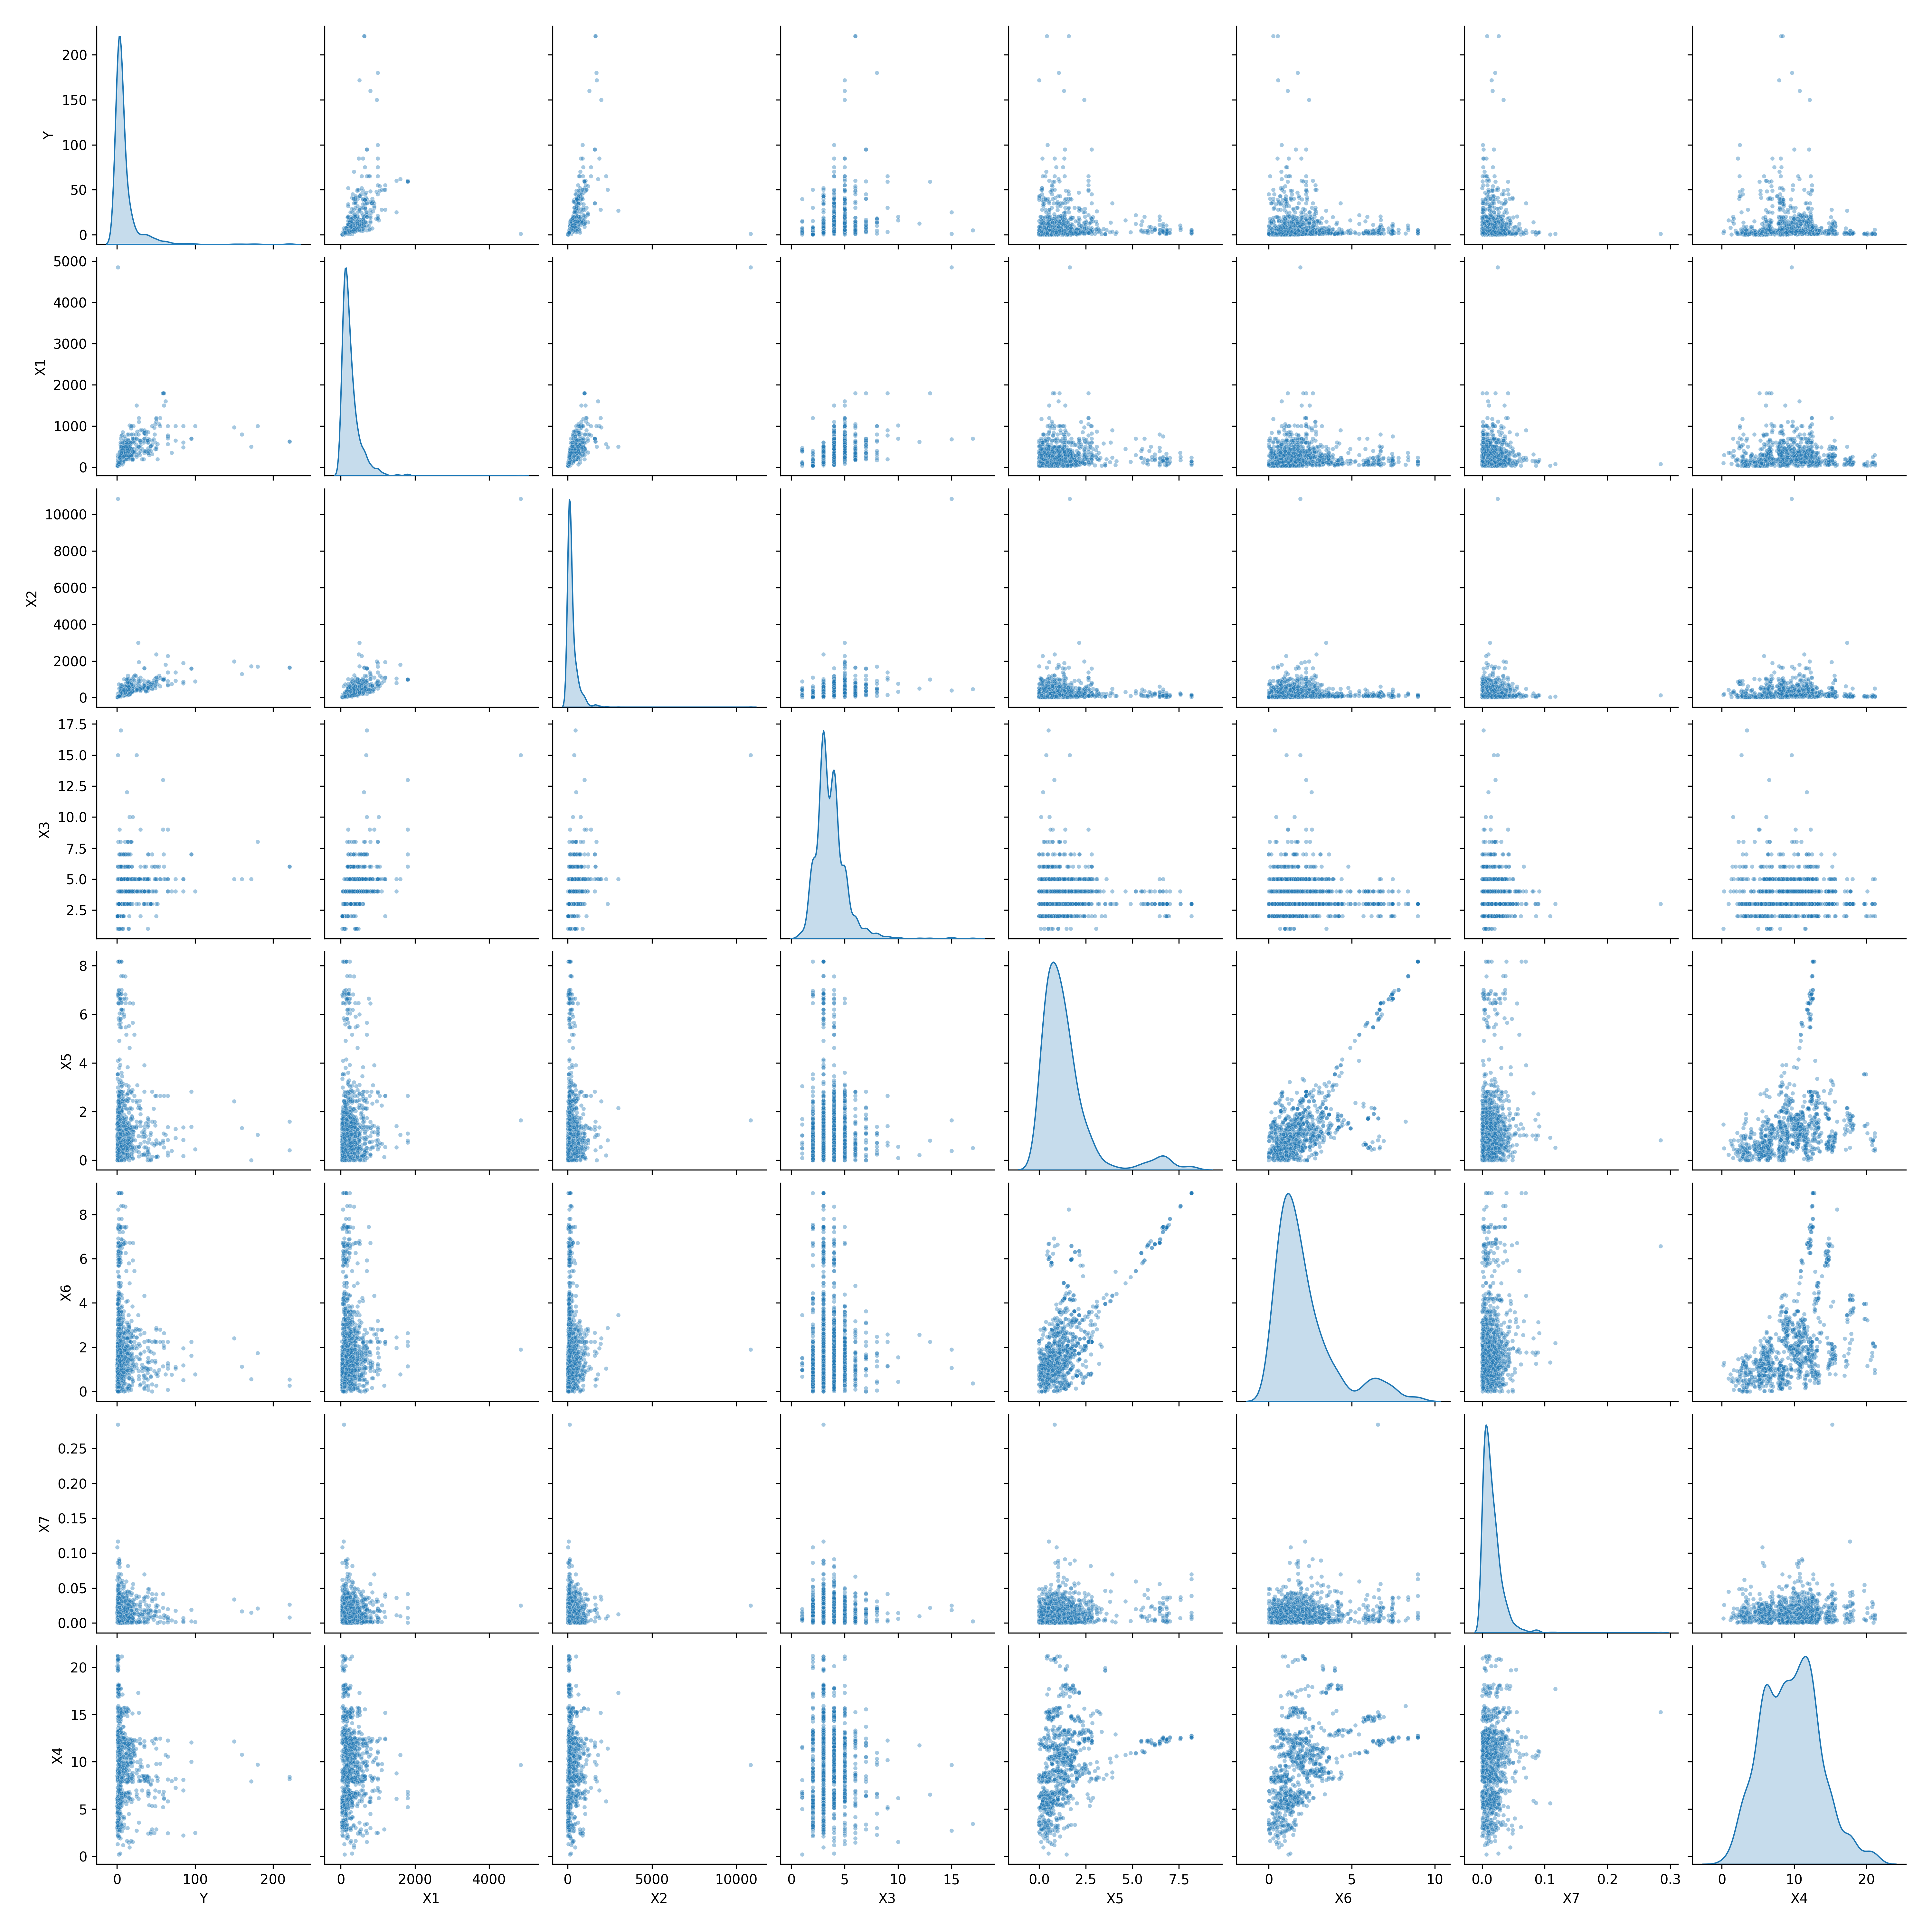
\includegraphics[width=\textwidth]{pairplot_deskriptif.png}
    \caption{Pairplot Matriks Hubungan Antar Variabel}
    \label{fig:pairplot_all}
\end{figure}

\newpage
%============================================================
\section{Analisis Pencilan (Outlier Analysis)}
%============================================================

Identifikasi pencilan dilakukan menggunakan metode \textit{Interquartile Range} (IQR) dengan batas $Q_1 - 1,5 \times IQR$ dan $Q_3 + 1,5 \times IQR$.

\begin{table}[H]
\centering
\caption{Identifikasi Jumlah dan Persentase Outlier per Variabel}
\label{tab:outliers}
\begin{tabular}{lrr}
\toprule
\rowcolor{headerblue}
\textcolor{white}{\textbf{Variabel}} & \textcolor{white}{\textbf{Jumlah Outlier}} & \textcolor{white}{\textbf{Persentase}} \\
\midrule
\rowcolor{rowlight}
Harga (Y) & 119 & 11.03\% \\
LB (X1) & 68 & 6.30\% \\
\rowcolor{rowlight}
LT (X2) & 109 & 10.10\% \\
KT (X3) & 91 & 8.43\% \\
\rowcolor{rowlight}
Monas (X4) & 5 & 0.46\% \\
Sekolah (X5) & 76 & 7.04\% \\
\rowcolor{rowlight}
RS (X6) & 100 & 9.27\% \\
Jalan (X7) & 39 & 3.61\% \\
\bottomrule
\end{tabular}
\end{table}

\noindent \textbf{Catatan Penanganan Outlier:} 
Variabel harga ($Y$) dan luas ($X_1, X_2$) memiliki persentase pencilan yang signifikan. Hal ini mencerminkan karakteristik pasar properti Jakarta di mana terdapat hunian sangat mewah yang jauh melampaui rata-rata. Dalam analisis GWR, pencilan ini seringkali menjadi poin ketertarikan (\textit{local interest}) untuk melihat variasi spasial yang ekstrem.

\newpage
%============================================================
\section{Analisis Korelasi Antar Variabel}
%============================================================

\subsection{Matriks Korelasi Pearson}

\begin{table}[H]
\centering
\caption{Matriks Korelasi Pearson Antar Variabel (dihitung dari data mentah)}
\label{tab:corr_full}
\scriptsize
\setlength{\tabcolsep}{5pt}
\begin{tabular}{lrrrrrrrr}
\toprule
\rowcolor{headerblue}
\textcolor{white}{\textbf{}} &
\textcolor{white}{\textbf{Y}} &
\textcolor{white}{\textbf{X1}} &
\textcolor{white}{\textbf{X2}} &
\textcolor{white}{\textbf{X3}} &
\textcolor{white}{\textbf{X4}} &
\textcolor{white}{\textbf{X5}} &
\textcolor{white}{\textbf{X6}} &
\textcolor{white}{\textbf{X7}} \\
\midrule
\rowcolor{rowlight}
Harga (Y) & \textit{1.0000} & \textbf{0.5389} & \textbf{0.5166} & 0.3389 & -0.0827 & -0.0454 & -0.1188 & 0.0087 \\
LB (X1) & \textbf{0.5389} & \textit{1.0000} & \textbf{0.7969} & \textbf{0.6042} & -0.0565 & 0.0080 & -0.0678 & 0.0161 \\
\rowcolor{rowlight}
LT (X2) & \textbf{0.5166} & \textbf{0.7969} & \textit{1.0000} & 0.4706 & 0.0068 & -0.0437 & -0.0705 & 0.0167 \\
KT (X3) & 0.3389 & \textbf{0.6042} & 0.4706 & \textit{1.0000} & -0.0532 & -0.0787 & -0.0903 & -0.0018 \\
\rowcolor{rowlight}
Monas (X4) & -0.0827 & -0.0565 & 0.0068 & -0.0532 & \textit{1.0000} & 0.3241 & 0.4738 & 0.0938 \\
Sekolah (X5) & -0.0454 & 0.0080 & -0.0437 & -0.0787 & 0.3241 & \textit{1.0000} & \textbf{0.7470} & 0.0624 \\
\rowcolor{rowlight}
RS (X6) & -0.1188 & -0.0678 & -0.0705 & -0.0903 & 0.4738 & \textbf{0.7470} & \textit{1.0000} & 0.0837 \\
Jalan (X7) & 0.0087 & 0.0161 & 0.0167 & -0.0018 & 0.0938 & 0.0624 & 0.0837 & \textit{1.0000} \\
\bottomrule
\multicolumn{9}{l}{\footnotesize \textbf{Tebal} = korelasi kuat ($|r|>0{,}5$)}
\end{tabular}
\end{table}

\subsection{Pasangan Korelasi Bermakna}

\begin{table}[H]
\centering
\caption{Pasangan Variabel dengan Korelasi Bermakna ($|r|\geq0{,}30$)}
\label{tab:corr_interp}
\small
\begin{tabular}{lrl}
\toprule
\rowcolor{headerblue}
\textcolor{white}{\textbf{Pasangan}} &
\textcolor{white}{\textbf{$r$ Pearson}} &
\textcolor{white}{\textbf{Interpretasi}} \\
\midrule
\rowcolor{rowlight}
Harga (Y)--LB (X1) & 0.5389 & Korelasi positif sedang \\
Harga (Y)--LT (X2) & 0.5166 & Korelasi positif sedang \\
\rowcolor{rowlight}
Harga (Y)--KT (X3) & 0.3389 & Korelasi positif lemah-sedang \\
LB (X1)--LT (X2) & 0.7969 & Korelasi positif kuat \\
\rowcolor{rowlight}
LB (X1)--KT (X3) & 0.6042 & Korelasi positif sedang \\
LT (X2)--KT (X3) & 0.4706 & Korelasi positif lemah-sedang \\
\rowcolor{rowlight}
Monas (X4)--Sekolah (X5) & 0.3241 & Korelasi positif lemah-sedang \\
Monas (X4)--RS (X6) & 0.4738 & Korelasi positif lemah-sedang \\
\rowcolor{rowlight}
Sekolah (X5)--RS (X6) & 0.7470 & Korelasi positif kuat \\
\bottomrule
\end{tabular}
\end{table}

\newpage
%============================================================
\section{Multikolinearitas dan VIF}
%============================================================

\subsection{Variance Inflation Factor (VIF)}
VIF mengukur seberapa besar varians dari koefisien regresi yang meningkat akibat adanya multikolinearitas.

\begin{table}[H]
\centering
\caption{Hasil Perhitungan Variance Inflation Factor (VIF)}
\label{tab:vif}
\begin{tabular}{lrl}
\toprule
\rowcolor{headerblue}
\textcolor{white}{\textbf{Variabel}} & \textcolor{white}{\textbf{Nilai VIF}} & \textcolor{white}{\textbf{Status}} \\
\midrule
\rowcolor{rowlight}
LB (X1) & 3.4751 & Aman \\
LT (X2) & 2.8030 & Aman \\
\rowcolor{rowlight}
KT (X3) & 1.5953 & Aman \\
Monas (X4) & 1.3139 & Aman \\
\rowcolor{rowlight}
Sekolah (X5) & 2.3227 & Aman \\
RS (X6) & 2.6454 & Aman \\
\rowcolor{rowlight}
Jalan (X7) & 1.0116 & Aman \\
\bottomrule
\end{tabular}
\end{table}

\subsection{Panduan Penanganan Korelasi Tinggi}
Berdasarkan nilai VIF dan matriks korelasi, jika ditemukan nilai VIF $> 10$ atau korelasi antar variabel independen $> 0{,}80$, beberapa langkah evaluasi yang dapat diambil adalah:

\begin{enumerate}
    \item \textbf{Eliminasi Variabel:} Menghapus salah satu variabel yang redundan (misal: antara Luas Bangunan dan Luas Tanah jika keduanya sangat korelasi).
    \item \textbf{Penggabungan (Rasio):} Mengubah variabel menjadi bentuk rasio, seperti Luas Bangunan per Jumlah Kamar.
    \item \textbf{Penelitian Spasial (GWR):} Pada model GWR, multikolinearitas lokal dapat terjadi secara dinamis. Jika multikolinearitas hanya terjadi di beberapa lokasi, variabel dapat tetap dipertahankan dengan catatan interpretasi pada wilayah tersebut dilakukan dengan hati-hati.
\end{enumerate}

\subsection{Temuan Utama Korelasi}

\begin{enumerate}
  \item \textbf{Fisik $\to$ Harga (Positif Kuat):}
    Luas Bangunan ($X_1$) memiliki korelasi Pearson tertinggi dengan harga
    ($r\approx0{,}54$), diikuti Luas Tanah ($X_2$, $r\approx0{,}52$) dan
    Jumlah Kamar ($X_3$, $r\approx0{,}34$). Konsisten dengan teori valuasi
    hedonis bahwa dimensi fisik menjadi faktor penentu utama.

  \item \textbf{Multikolinearitas Fisik:}
    Korelasi sangat kuat antara $X_1$--$X_2$ ($r\approx0{,}80$) dan
    $X_1$--$X_3$ ($r\approx0{,}60$) mengindikasikan potensi
    \textit{multikolinearitas} dalam model OLS global.

  \item \textbf{Fasilitas Publik Terklasterisasi:}
    Korelasi $X_5$--$X_6$ ($r\approx0{,}75$) sangat tinggi --- sekolah dan
    rumah sakit cenderung berlokasi berdekatan, mengkonfirmasi pola zonasi
    fasilitas publik di Jakarta.

  \item \textbf{Jarak Negatif ke Harga:}
    $X_4$ dan $X_6$ berkorelasi negatif dengan $Y$, meski lemah secara global.
    Heterogenitas spasialnya dikaptulasi lebih baik oleh model GWR lokal.

  \item \textbf{Jalan Utama Hampir Tidak Berkorelasi:}
    $X_7$ memiliki korelasi mendekati nol dengan $Y$ ($r\approx0{,}009$),
    kemungkinan karena hampir semua properti memiliki akses jalan yang setara.
\end{enumerate}

\newpage
%============================================================
\section{Catatan Metodologis}
%============================================================

\subsection{Rumus yang Digunakan}

Seluruh ukuran statistik deskriptif dihitung menggunakan formula standar berikut:

\begin{align*}
\text{Rata-rata:} \quad & \bar{x} = \frac{1}{n} \sum_{i=1}^{n} x_i \\[6pt]
\text{Varian (tidak bias):} \quad & s^2 = \frac{1}{n-1} \sum_{i=1}^{n} (x_i - \bar{x})^2 \\[6pt]
\text{Koef. Variasi:} \quad & \text{CV} = \frac{s}{|\bar{x}|} \times 100\% \\[6pt]
\text{Skewness (Fisher):} \quad & g_1 = \frac{n}{(n-1)(n-2)} \sum_{i=1}^{n} \left(\frac{x_i - \bar{x}}{s}\right)^3 \\[6pt]
\text{Excess Kurtosis:} \quad & g_2 = \frac{n(n+1)}{(n-1)(n-2)(n-3)} \sum_{i=1}^{n}\left(\frac{x_i-\bar{x}}{s}\right)^4 \\
& \quad - \frac{3(n-1)^2}{(n-2)(n-3)} \\[6pt]
\text{Korelasi Pearson:} \quad & r_{XY} = \frac{\sum_{i=1}^{n}(x_i-\bar{x})(y_i-\bar{y})}
  {\sqrt{\sum_{i=1}^{n}(x_i-\bar{x})^2}\;\sqrt{\sum_{i=1}^{n}(y_i-\bar{y})^2}} \\[6pt]
\text{IQR:} \quad & \text{IQR} = Q_3 - Q_1 \\[6pt]
\text{Persentil (Interp.\ Linear):} \quad & P_p = x_{(L)} + \text{frac}\cdot(x_{(L+1)}-x_{(L)})
\end{align*}

\subsection{Catatan Implementasi}
\begin{itemize}
  \item Varian dihitung dengan \textit{estimator tidak bias} (pembagi $n-1$).
  \item Skewness dan kurtosis menggunakan koreksi Fisher--Pearson (\textit{adjusted}).
  \item Persentil menggunakan metode interpolasi linear.
  \item Data diekstrak langsung dari \texttt{rumah\_27\_8\_25\_clean.geojson} tanpa transformasi.
\end{itemize}

\newpage
%============================================================
\section{Lampiran: Akses Data Penelitian}
%============================================================

Seluruh dataset primer yang digunakan dalam analisis ini, mencakup file GeoJSON mentah,
dataset Excel hasil pembersihan, serta script pemrosesan data, dapat diakses
melalui repositori daring berikut:

\begin{center}
\textbf{Link Dataset (Google Drive):}\\
{\raggedright \url{https://drive.google.com/drive/folders/1dmIp66Qh8gmt7BZdckrE9OWTKQKyhDJV?usp=sharing} \par}
\end{center}

Dataset ini disediakan untuk kepentingan replikasi penelitian dan transparansi
metodologi pemodelan spasial.

\end{document}
